\chapter{Workspace Manager}

Workspace manager encapsulates all functionality of the parser library. It is the access point to all parsing capabilities, keeps the current state of all open files and resolves libraries needed by the analyzer. It also manages when files should be reparsed.

\section{Parser library API}

First of all, the workspace manager component is the only public interface of the parser library. The API design is based on LSP and DAP, most of the API is just LSP/DAP rewritten in C++. The API uses the observer pattern for DAP events and notifications originating in parser library (e.g. textDocument/publishDiagnostics).

The API can be divided into three categories:
\begin{itemize}
	\item Editor state and file content synchronization (\cref{text_sync_methods})
	\item Parsing results presentation 
	\item Macro tracer
\end{itemize}

\subsection{Editor state and file content synchronization}

\begin{table}
	\centering
	\begin{tabular}{ll}
		
		\toprule
		Method & Description \\ \midrule
		did\_open (file name, file content) & \multirow{3}{8cm}{Three methods that are called whenever the user opens a file, changes contents of an already opened file or closes a file in the editor.} \\
		did\_change (file name, changes)& \\
		did\_close (file name)& \\
		& \\
		\multirow{3}{5cm}{did\_change\_watched\_files(file paths)} &\multirow{3}{8cm}{Method, that is called when a file from a workspace has been changed outsize of the editor} \\
		& \\
		& \\
		& \\
		add\_workspace (ws name, ws path) & \multirow{2}{8cm}{Methods that are called when the user opens or closes a workspace in the editor} \\
		remove\_workspace (ws path) & \\ \bottomrule
	\end{tabular}
	
	\caption{List of all Editor state and text synchronization methods}
	\label{text_sync_methods}
\end{table}

All the methods from the first category are listed in \cref{text_sync_methods}. There are two types of files that need to be synchronised:
\begin{itemize}
	\item Files, that the user has opened in the editor. Those files are being edited by the user and their content may be different from the files actually saved in the filesystem.
	\item Files, that the parser library opens from the hard disk, because they are needed to parse opened files (e.g. a macro that is used by an opened file)
\end{itemize}

So the parser library is allowed to load arbitrary files from the disk, and use its contents until such file is opened in the editor. From that point on, the only source of truth for the contents of the file are the did\_change notifications. Once the file is closed in the editor, the parser library is again allowed to rely on its contents in the filesystem.



\subsection{Parsing results presentation}

\begin{table}
	\centering
	\begin{tabular}{ll}
		
		\toprule
		Method & Description \\ \midrule
		& \multirow{3}{8cm}{The method gets a position in an opened file. If there is a symbol, the method returns position of definition of that symbol} \\
		definition(file name, caret position) &  \\
		& \\
		& \\
		& \multirow{3}{8cm}{The method gets a position in an opened file. If there is a symbol, the method returns list of positions where the symbol is used}\\
		references(file name, caret position) & \\
		& \\
		& \\
		& \multirow{3}{8cm}{The method gets a position in an opened file where the user points with cursor. Returns list of strings to be shown in a tooltip window}\\
		hover(file name, mouse position)& \\
		& \\
		& \\
		& \multirow{3}{8cm}{The method gets a position in an opened file and how the completion box was triggered (i. e. with what key, automatically/manually). Returns list of strings suggested for completion at the position}\\
		completion(file name,& \\
		mouse position, trigger info)& \\
		& \\
		& \\ \bottomrule
	\end{tabular}
	
	\caption{List of all parse results methods}
	\label{parse_results}
\end{table}

All the methods from the second category are listed in \cref{parse_results}. They get position of caret or mouse cursor in a file and are expected to return information about the place in code. For example method \TT{hover} is called when the user points at some word in the code and waits for a short time. The method returns a string that the editor shows in tooltip window at the position. Typically, the tooltip would show type of a variable and its value, if known.

Additionally, the parser library presents its results using the observer pattern. There are two interfaces: highligting and diagnostics consumer. Each of them has method \TT{consume} that gets updated information as parameter whenever there is an update. Any potential user of the library (e.g. the language server component) just has to implement the interfaces to process the results.

\subsection{Macro tracer}
\todo{probably move this table to macro tracer section. Just brief summary of macro tracer API here.}
\begin{table}
	\centering
	\begin{tabular}{ll}
		
		\toprule
		Method & Description \\ \midrule
		launch(file name) & Starts the macro tracer \\
	    next() & Method called when the user triggered step over. \\
		step\_in() & Method called when the user triggered step in. \\
		disconnect() & Method called when the user stopped macro tracer \\
		continue\_debug() & \multirow{2}{8cm}{Method called when the user wants to continue to next breakpoint} \\
		& \\
		
		get\_stack\_frames() & Returns list of all stack frames\\
		get\_scopes(frame ID) & Returns list of scopes for given stack frame \\
		get\_variable(variable reference) & Returns list of variables  \\
		
		
		set\_breakpoints (file name,
		list of lines) & Sets breakpoints to specified lines of a file \\ \bottomrule
	\end{tabular}
	
	\caption{List of all parse results methods}
	\label{macro_tracer_API}
\end{table}


The macro tracer part of the API is again just DAP rewritten in C++. All the methods are listed in \cref{macro_tracer_API}. There are methods that are called when the user clicks on buttons to control the macro tracer: launch the tracer, step in, step over, continue and stop. Moreover, there are methods that retrieve information about current state of traced code: stack of macro calls and information about compile time variables.

\section{Architecture overview}

\begin{landscape}
\begin{figure}
	\centering
	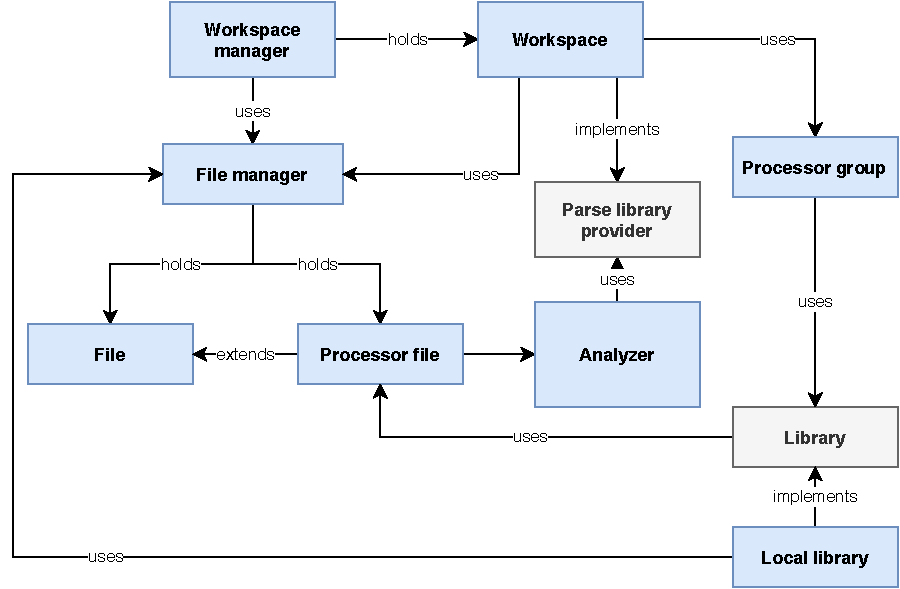
\includegraphics[width=16cm]{img/ws_mngr_arch}
	\caption{Architecture of workspace manager.}
	\label{ws_mngr_arch}
\end{figure}
\end{landscape}
\section{Files}




\section{Libraries resolution}

\section{Diagnosable}